\numberwithin{figure}{section}

%----------------------------------------------------------------------------
\chapter{Háttér ismeretek}
%----------------------------------------------------------------------------
\section{Modern technológiák}
%----------------------------------------------------------------------------

A megoldás folyamán számos modern technológia bevezetésére, implementációjára volt szükség,  ezek közül a legfontosabbak:

%----------------------------------------------------------------------------
\subsection{OSGi}
%----------------------------------------------------------------------------

Az OSGi (Open Services Gateway Initiative) egy Java keretrendszer, amely segítségével moduláris szoftvereket és könyvtárakat tudunk fejleszteni.

A technológia alapvetően egy specifikáció halmazból, referencia implementációkból és minden specifikációhoz tartozó teszt halmazból áll össze, mindezek együtt leírnak egy dinamikus moduláris rendszert. A bevált szolgáltatás modellje lehetővé teszi, hogy az infrastruktúra és az alkalmazás komponensek úgy lokálisan, mint hálózaton keresztül is kommunikáljanak egymással, hogy egy koherens és konzisztens architektúrát alkossanak.

Az ipar bármely területén megtaláljuk az IoT-tól kezdve a telekommunikációs megoldásokig, viszont számos esetben nincs kiemelve, azaz ritkán van feltüntetve a használt technológiák listáján. 

Kompozícióilag két részből áll az OSGi. Az első egy olyan specifikáció, ami a moduláris egységeket írja le, ezeket bundle-knek vagy plug-in-eknek nevezzük. A specifikáció leírja, hogy milyen infrastruktúra szükséges az említett bundle-k számára és, hogy egyes bundle-k milyen életcikluson mennek át (Telepítve, Elindítva, Aktív, Elakadt, Felfüggesztett), továbbá meghatározza, hogy milyen kapcsolat lehet egyesek bundle-k közt és ezek hogyan kommunikálhatnak egymással. A második pedig egy JVM szintű nyilvántartó, amibe minden bundle tud bejegyzéseket tenni, hogy neki milyen publikálni kívánt objektumai vannak.


Az OSGi a fejlesztési ciklus majdnem minden területén csökkenti a komplexitást. Kódírás és tesztelés jelentősen kevesebb erőforrást fog elnyelni, támogatja az újrahasznosítást (létező komponenseket egyszerűen fel lehet használni egy új modulban). Az üzemeltetési feladatokat is könnyíti, lehetővé teszi a moduláris frissítést vagy telepítést, nem kell minden funkció bevezetésekor az egész rendszert leállítani. Könnyebben lehet lokalizálni egyes hibákat, így a támogatói feladatkör is egyszerűsödik. Az alkalmazásunk moduláris függőségi fájában egyszerűbben tudunk bizonyos elemeket bevezetni, helyettesíteni vagy akár kivenni.

További részletes leírást az OSGi specifikációban lehet olvasni:  \textbf{\href{https://www.osgi.org/developer/specifications/}{OSGi Specification}}

Eclipse világban az Equinox OSGi implementációt lehet használni, a fentebb részletezett szolgáltatásokat és szükséges infrastruktúrát alakítja ki számunkra.

%----------------------------------------------------------------------------
\subsection{Eclipse Plug-in fejlesztés}
%----------------------------------------------------------------------------

Eclipse egy nyílt forráskódú, platform független fejlesztői környezet (IDE). Egy alap munkaterület (workspace) és egy plug-in rendszert tartalmaz, aminek segítségével könnyen tesztre szabhatóvá lehet tenni. Az utóbbit használja ki a Gamma is és az általa használt mellék komponensek is. 

Az Eclipse IDE egy speciális Eclipse alkalmazás ami lehetővé teszi a fejlesztőknek, hogy egyedi alkalmazásokat tudjanak fejleszteni. Egy Eclipse alkalmazás egy vagy több szoftver komponensből tevődik össze ezeket nevezünk plug-in-eknek. Ezek a modulok bővíthetőek vagy felhasználhatóak más komponensek létrehozására. Összefoglalva, az Eclipse IDE egy több plug-in-ekből (JDT) álló Eclipse alkalmazás.

Lehetőségünk van az így létrehozott alkalmazásainkat összecsomagolni és az Eclipse IDE- től függetlenül futtatni és tesztelni.
Ehhez definiálnunk kell egy termék leírást (product configuration), aminek tartalmaznia kell az alkalmazásunk plug-in-jét, minden felhasznált függőséget és minden más olyan konfigurációt ami szükséges ahhoz, hogy egy külön komponenseként tudjuk hordozni a szoftverünket. Ilyen konfigurációk, az alkalmazás belépési pontja (extension point), komponensek indulási sorrendje, esetleges ikonok és függőségi fa, ami meghatározza, hogy milyen komponens mitől és hogyan (kötelező, opcionális) függ valamilyen más modultól.

A termékleírásunk egy alkalmazás osztályra kell mutasson ami alapértelmezetten két fajta lehet:

\begin{lstlisting}[language=]
org.eclipse.ui.ide.workbench - IDE alapú alkalamzások

org.eclipse.e4.ui.workbench.swt.E4Application - RCP alkalmazások, függetlenek az IDE-től
\end{lstlisting}

Ezektől el lehet térni és egy teljesen egyedi alkalmazást írni, ehhez a következő interfészt kell implementálni és behivatkozni a termék konfigurációnkba :

\begin{lstlisting}[language=]
org.eclipse.equinox.app.IApplication
\end{lstlisting}

A dolgozatban leírt fejlesztés ezzel a megoldási opcióval lett megvalósítva.

%----------------------------------------------------------------------------
\subsection{REST API}
%----------------------------------------------------------------------------

Az internet megszületése óta, mikor Charley Kline és Bill Duvall összekötöttek két számítógépet és elküldték egymásnak az "L" és "O" karaktereket, számos internet alapú adatmozgatási megoldás született ilyenek a CORBA, RPC vagy SOAP. Ezek mind nagyon komplex mechanizmusok és a mai világban elavultnak számítanak. Itt jön szóba a REST a legújabb iteráció az internetes adatszállítási megoldások körében.

REST vagy \textbf{RE}presentational \textbf{S}tate \textbf{T}ransfer egy tervezési stílus, amellyel különböző rendszerek közti kapcsolatot tudunk megvalósítani. Olyan rendszereket, amelyek megfelelnek a REST szabványnak RESTful rendszereknek is nevezünk, alapvetően ezeket két fő jellemző írja le, az első, hogy nem tartják nyilván az egyes kérések állapotát, a második pedig az, hogy elkülönítik a kliens és szerver fogalmakat. 

\begin{figure}[!ht]
	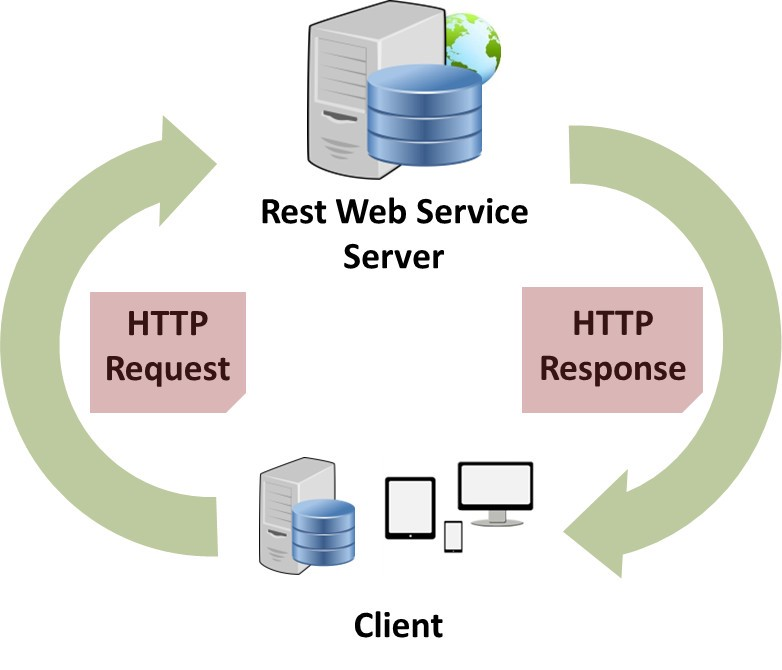
\includegraphics[width=150mm, keepaspectratio]{figures/rest_structure.jpeg}
	\caption{REST egyszerű architektúra}
	\label{fig:rest_structure}
\end{figure}

Ahhoz, hogy egy szolgáltatást RESTful-nak nevezzünk meg kell felelni egy szabványnak ami hat alapelvből áll.

 \begin{itemize}
	\item \textbf{Szerver és Kliens szeparáció} - a tervezési minta előírja, hogy a szerver és a kliens két független és önállóan egységként létező komponens kell legyen. Ez lehetővé teszi, hogy a két rendszerünket külön tudjuk fejleszteni, telepíteni, javítani, karban tartani. Bármilyen kódmódosítást kell végezni bármelyik oldalon a másikat nem befolyásolja mind addig amíg az interfész nem módosul, ilyenkor a szerver egy master szerepet vesz át és az elvégzett módosítást kezelni kell kliens oldalon is. Ez az elv támogatja a moduláris gondolkodást, ezzel flexibilissé válik a komplex rendszerünk. Továbbá, skálázhatósági lehetőségek is felmerülnek, hiszen az erőforrás igényesebb komponens alatti erőforrásokat igény szerint bővíthetjük. A szétválasztás lehetővé teszi, hogy akár egy szerverhez több kliens is csatlakozzon, így sokszínű rendszereket tudunk létrehozni. Ennek egy vizuális reprezentációja \aref{fig:rest_structure} ábrán látható.
	\item \textbf{Állapot nélküliség} - Ez az alapelv annyit von magában, hogy a szerver semmilyen információval nem rendelkezhet a kliens állapotáról ennek a kijelentésnek viszont fordítva is teljesülnie kell, azaz a kliens se ismerheti a szerver állapotát. Minden küldött/kapott üzenet egységként lehet kezelni, független attól, hogy a múltban milyen jellegű üzenet váltások történtek. Ennek eredménye az, hogy a csak kliens tárolja a saját adatainak az állapotát (nem a szerver adatait).
	\item \textbf{Egységes interfész} - Ez az alapelv négy szabályt határoz meg:
	\begin{enumerate}
		\item A kliens által kezdeményezett kérésnek tartalmaznia kell a fent definiált erőforrásnak az azonosítóját. Az erőforrást (egyed/objektum) hívhatjuk a webes kontextus alanyának is.
		\item A szerver válasza elegendő információt kell tartalmazzon az erőforrásról, pontosabban annyit, hogy a kliens tudja majd módosítani ezt.
		\item Minden egyes hívás az API felé részletes és tartalmilag teljes kell legyen. Továbbá a szerver válaszának is tartalmaznia kell elegendő információt, úgy, hogy a kliens értelmezni tudja ezt.
		\item Az utolsó szabálytól gyakran eltekintenek a fejlesztők, ez azt mondja, hogy a válasz, ami a szervertől érkezik tartalmazhat, olyan útmutatókat a kliens számára amivel az alkalmazás állapotát módosítani tudja. Például, ha egy objektumot lekér a kliens az API-tól, akkor a szerver a válaszba becsomagolhat olyan mellékes információkat amelyek azt írják le, hogy milyen módon módosítható a visszaadott objektum.
	\end{enumerate}
	Az egységes interfész lehetővé teszi, hogy a kliens típusától (böngésző, alkalmazás) eltudjunk tekinteni a szerver oldalon.
	\item \textbf{Cache lehetőség} - Cache támogatást úgy lehet elérni, hogy az adatokat verziózzuk, ha a kliens lekér egy adatot akkor valamilyen metaadatban tároljuk azt is, hogy ez milyen verziójú, így ha ugyanazt az objektumot szeretné lekérni, előtte tudja ellenőrizni lokálisan, hogy már a legfrissebb adattal rendelkezik és nem kell a szervert megint megszólítania. Ezzel terheléscsökkentést tudunk elérni.
	\item \textbf{Rétegelt architektúra} - A szerver és az erőforrást lekérő kliens között számos más rendszer helyezkedhet el, ezek többfajták lehetnek de legtöbbször a biztonsági, cache, terhelés egyensúlyozó rétegekkel találkozhatunk.
	\item \textbf{Igény szerinti kód (opcionális)} - Az egyedüli elv ami opcionális, annyit von magában, hogy a kliens bármikor kérhet kódrészleteket a szervertől és ez a válaszban valamilyen HTML vagy szkript formátumba becsomagolja és elküldi ennek , amit majd a kliens futtatni tud. Az alapelv teljesülése nélkül is tud egy rendszer RESTful lenni.
\end{itemize}

A fentebb többször említett kérés/válasz fogalmakat a REST világban HTTP kérésekbe csomagoljuk, ezek tipikusan a következőket kell tartalmazzák :
\begin{enumerate}
	\item egy HTTP ige, ami leírja a művelet típusát, jelenleg használt igék:
	\begin{enumerate}
		\item \textbf{GET} erőforrást tudunk lekérni, nagyon fontos, hogy nem módosíthat állapotot a szerveren
		\item \textbf{POST} erőforrás létrehozásra használják, többszörös hívás esetén különböző erőforrásokat fog létrehozni
		\item \textbf{PUT} már létező erőforrások állapot frissítésére használják, többszörös hívás ugyanazt kell, hogy eredményezze
		\item \textbf{DELETE} mint ahogy a neve is sugallja, erőforrás törlésre használják 
		\item \textbf{PATCH} parciális frissítési műveletekre tudjuk használni
		\item a maradék HTTP igéket nem szokták gyakran implementálni a REST világban
	\end{enumerate} 
	\item fejléc, ami metaadatokat tartalmaz az üzenetről, többek közt olyan jellegű információkat, mint az üzenet hossza, a tartalom típusa, a válasz HTTP kód száma és üzenete.
	\item az erőforrás elérési útja
	\item opcionális üzenettörzs, ami további adatot tartalmazhat
\end{enumerate}


%----------------------------------------------------------------------------
\subsection{OpenAPI}
%----------------------------------------------------------------------------

%----------------------------------------------------------------------------
\subsection{Fontosabb Java könyvtárak}
%----------------------------------------------------------------------------

%----------------------------------------------------------------------------
\section{Gamma}
%----------------------------------------------------------------------------









